\documentclass[border=2pt]{standalone}
\usepackage{amsmath}
\usepackage{pgfplots}
\pgfplotsset{compat=1.18}
\begin{document}
\footnotesize
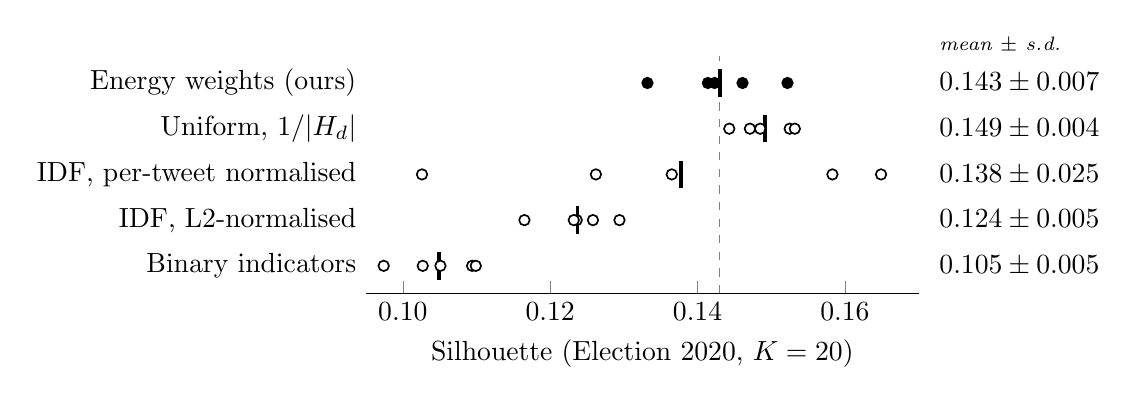
\begin{tikzpicture}
\begin{axis}[width=8.6cm, height=4.6cm, scale only axis=false,
  xmin=0.095, xmax=0.170, ymin=-0.6, ymax=4.6,
  xtick={0.10,0.12,0.14,0.16}, xticklabel style={/pgf/number format/fixed,/pgf/number format/precision=2,/pgf/number format/fixed zerofill},
  ytick={0,1,2,3,4}, yticklabels={{Binary indicators},{IDF, L2-normalised},{IDF, per-tweet normalised},{Uniform, $1/|H_d|$},{Energy weights (ours)}},
  axis y line*=left, axis x line*=bottom, y axis line style={draw=none}, ytick style={draw=none},
  xlabel={Silhouette (Election 2020, $K=20$)}, clip=false]
\draw[gray, dashed, line width=0.5pt] (axis cs:0.1430,-0.6) -- (axis cs:0.1430,4.6);

\addplot[only marks, mark=*, mark size=1.9pt, mark options={fill=black, draw=black, line width=0.6pt}] coordinates {(0.1522,4) (0.1461,4) (0.1332,4) (0.1414,4) (0.1423,4)};
\draw[line width=1.4pt] (axis cs:0.1430,3.70) -- (axis cs:0.1430,4.30);
\node[anchor=west] at (axis cs:0.1715,4) {$0.143 \pm 0.007$};
\addplot[only marks, mark=*, mark size=1.9pt, mark options={fill=white, draw=black, line width=0.6pt}] coordinates {(0.1471,3) (0.1443,3) (0.1525,3) (0.1532,3) (0.1485,3)};
\draw[line width=1.4pt] (axis cs:0.1491,2.70) -- (axis cs:0.1491,3.30);
\node[anchor=west] at (axis cs:0.1715,3) {$0.149 \pm 0.004$};
\addplot[only marks, mark=*, mark size=1.9pt, mark options={fill=white, draw=black, line width=0.6pt}] coordinates {(0.1262,2) (0.1583,2) (0.1649,2) (0.1365,2) (0.1026,2)};
\draw[line width=1.4pt] (axis cs:0.1377,1.70) -- (axis cs:0.1377,2.30);
\node[anchor=west] at (axis cs:0.1715,2) {$0.138 \pm 0.025$};
\addplot[only marks, mark=*, mark size=1.9pt, mark options={fill=white, draw=black, line width=0.6pt}] coordinates {(0.1165,1) (0.1294,1) (0.1236,1) (0.1232,1) (0.1258,1)};
\draw[line width=1.4pt] (axis cs:0.1237,0.70) -- (axis cs:0.1237,1.30);
\node[anchor=west] at (axis cs:0.1715,1) {$0.124 \pm 0.005$};
\addplot[only marks, mark=*, mark size=1.9pt, mark options={fill=white, draw=black, line width=0.6pt}] coordinates {(0.1094,0) (0.1051,0) (0.1099,0) (0.0974,0) (0.1027,0)};
\draw[line width=1.4pt] (axis cs:0.1049,-0.30) -- (axis cs:0.1049,0.30);
\node[anchor=west] at (axis cs:0.1715,0) {$0.105 \pm 0.005$};
\node[anchor=south west, font=\scriptsize\itshape] at (axis cs:0.1715,4.45) {mean $\pm$ s.d.};
\end{axis}
\end{tikzpicture}
\end{document}